\bookchapter{Capitolo 37: La rivoluzione di paradigma — da «scrivere codice» a «dire all'AI di scrivere codice»}

\chapterintro{Congratulazioni: aprendo questo libro ti trovi al centro di una rivoluzione professionale. Il punto di partenza è una frase pubblicata sui social da un programmatore nel 2025. Sembra drammatico? Ma è andata proprio così.}

\booksection{La nascita del Vibe Coding: un movimento nato da una frase}

Nel febbraio 2025 Andrej Karpathy — ricorda questo nome, lo incontrerai ancora — pubblicò un tweet poi citato innumerevoli volte: «C'è un nuovo modo di programmare che chiamo Vibe Coding: vai completamente a sensazione (vibes), ignora i dettagli del codice e lascia che l'AI faccia tutto. Dici quello che vedi, copi e incolli, basta che funzioni.»

Quella frase apparentemente casuale diede in realtà un nome preciso a un cambiamento di paradigma già in corso: gli umani non scrivono più codice riga per riga, ma descrivono l'intenzione in linguaggio naturale e l'AI realizza l'implementazione. Il tono di Karpathy era scherzoso, ma l'intuizione era profonda: quando la capacità di generazione del codice da parte dell'AI supera una certa soglia, il collo di bottiglia non è più «riesco a scrivere questa riga?», ma «riesco a pensare con chiarezza cosa voglio?».

\begin{tcbinfo}{Suggerimento: cos'è un «vibe»?}
Vibe significa letteralmente «atmosfera, sensazione». Il Vibe Coding è «programmare con l'AI seguendo le sensazioni»: descrivi ciò che vuoi e l'AI lo realizza. Ricorda questa parola: è l'atto di nascita di questa rivoluzione.

\end{tcbinfo}

Da quel momento il significato di «codifica» si è diviso: quella traduzionale traduce il design in sintassi; quella nuova traduce l'intenzione in istruzioni. La prima mette alla prova le dita, la seconda il cervello.

Il termine Vibe Coding passò rapidamente da scherzo a concetto ingegneristico serio. A metà 2026 si era già evoluto in un'intera metodologia — dalla espressione dei requisiti alla gestione del contesto, dall'iterazione e verifica alla qualità. Si capì anche che «seguire le sensazioni» è solo lo stadio iniziale: la programmazione AI efficiente richiede un pensiero sistematico. Ed è esattamente ciò che questo libro ti offre.

\booksection{Stato dell'arte nel 2026: l'era dell'Agentic Engineering}

Ad agosto 2026 la programmazione AI aveva già attraversato diverse iterazioni di paradigma. Il Vibe Coding fu la prima scintilla, ma presto ci si rese conto che «parlare a sensazione» con l'AI produceva codice di qualità instabile — a volte brillante, a volte disastroso. Il paradigma evolse: dalla semplice programmazione conversazionale all'ingegneria strutturata degli Agent.

Ancora Karpathy, all'inizio del 2026, propose il concetto di Agentic Engineering. A differenza del Vibe Coding «dimmi e genero», l'Agentic Engineering sottolinea: dai un obiettivo all'AI, lascia che pianifichi i passaggi, chiami strumenti, verifichi i risultati e iteri le correzioni. L'AI non è più un semplice generatore di codice, ma un agente che percepisce l'ambiente, prende decisioni ed esegue azioni.

Questo passaggio ha portato tre cambiamenti chiave:

\begin{enumerate}
  \item Modalità di interazione: da «domanda-risposta» a «imposta l'obiettivo e delega».
  \item Prodotto del lavoro: da «un pezzo di codice» a «un progetto completo».
  \item Ruolo umano: da «revisionare il codice riga per riga» a «definire i confini, validare i risultati».
\end{enumerate}

I numeri non mentono: con Cursor 3, rilasciato ad aprile 2026, l'uso della modalità Agent superò per la prima volta quella di completamento Tab, segnando la svolta di massa degli sviluppatori; Claude Code, lo strumento di programmazione AI nativo da terminale, raggiunse a metà 2026 un fatturato annuo di 2,5 miliardi di dollari. Il grafico seguente mostra questo momento di incrocio:

\begin{center}
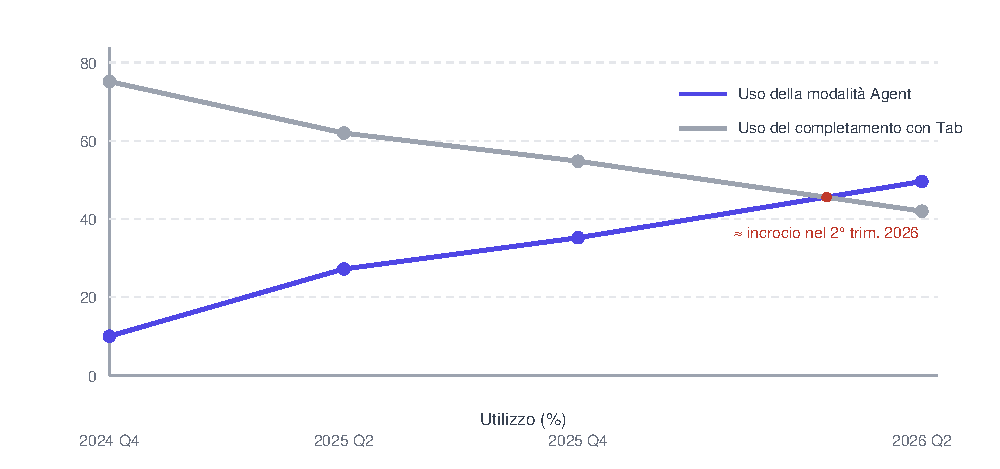
\includegraphics[width=0.92\linewidth]{figures/fig-di-san-shi-qi-zhang-1}
\\[2pt]\small Figura 1: andamento dell'uso delle modalità di interazione nella programmazione AI (stime da ricerche di settore; nel Q2 2026 la modalità Agent supera il completamento Tab)
\end{center}

Ma diciamolo chiaramente: i cambiamenti di strumenti e modelli sono solo la superficie. Che tu usi Cursor o Claude Code, che il modello sia GPT-5 o Claude 4.5, i praticanti di successo della programmazione AI seguono la stessa metodologia di base. Ed è ciò che questa guida ti insegna.

\booksection{Il cambiamento cognitivo: da Coder a Conductor}

L'educazione tradizionale alla programmazione ti insegna a diventare un Coder: comprendere la sintassi, memorizzare le API, fare debug. Nell'era della programmazione AI questo ruolo viene ridefinito. Non devi più scrivere riga per riga, ma devi diventare un «comandante» (Conductor): definire il campo di battaglia, stabilire le regole, assegnare i compiti, validare i risultati.

Il cuore del cambiamento non è «sai scrivere codice?», ma «sai pensare con chiarezza cosa fare?». Un ottimo comandante non è necessariamente il miglior soldato, ma deve conoscere meglio di tutti obiettivo, terreno e schieramento. Allo stesso modo, un buon praticante di programmazione AI non padroneggia ogni dettaglio di sintassi, ma conosce bene obiettivi del progetto, vincoli architetturali e standard di qualità.

Questa tabella merita di essere letta due volte: riassume tutto il cambiamento di ruolo:

\begin{center}
\begin{tabularx}{\linewidth}{|X|X|X|}
\hline
\textbf{Dimensione} & \textbf{Coder tradizionale} & \textbf{Comandante AI (Conductor)} \tabularnewline
\hline
Competenze chiave & Memoria della sintassi, chiamate API, debug & Definizione dei requisiti, gestione del contesto, giudizio di accettazione \tabularnewline
Modalità di lavoro & Scrivere codice riga per riga & Descrivere l'intenzione, revisionare l'output \tabularnewline
Controllo qualità & Se l'ho scritto io, lo so come è fatto & Verificare l'output dell'AI con test e revisioni \tabularnewline
Requisiti di conoscenza & Padroneggiare in profondità un linguaggio/framework & Comprendere ampiamente il panorama tecnico e in profondità la logica di business \tabularnewline
Dove sta il collo di bottiglia & Velocità di codifica e memoria della sintassi & Chiarezza del pensiero e capacità espressiva \tabularnewline
Origine degli errori & Errori di sintassi, omissioni logiche & Requisiti ambigui, contesto insufficiente \tabularnewline
\hline
\end{tabularx}
\end{center}

\begin{center}\small\color{gray}Confronto tra Coder tradizionale e comandante AI\end{center}

Questo non significa che la conoscenza della programmazione non conti. Al contrario: solo se capisci il codice scritto dall'AI puoi revisionarlo e correggerlo efficacemente; solo se comprendi strutture dati e algoritmi puoi giudicare se la soluzione dell'AI è sensata. La tua riserva di conoscenza determina il «tetto del tuo comando» — ma il ruolo della conoscenza passa da «strumento di esecuzione» a «base di giudizio».

\booksection{Perché la metodologia conta più degli strumenti}

Gli strumenti si rinnovano ogni tre mesi, la metodologia evolve solo ogni tre anni. Impari le meccaniche di uno strumento e tra tre mesi potrebbe essere superato; padroneggi un modo di pensare e tra tre anni vale ancora.

Chi inizia con la programmazione AI spesso chiede subito «qual è il miglior strumento» o «qual è il modello più forte». Domande legittime, ma con le priorità sbagliate. Lo scenario degli strumenti ad agosto 2026 è completamente diverso da quello di agosto 2025: Trae, Qoder e altri sono saliti e scesi, Cursor è passato da plugin a IDE indipendente fino a Cursor 3, Claude Code da progetto sperimentale a scelta principale per la programmazione da terminale. Ma dietro questi cambiamenti, i principi di pensiero dei praticanti di successo sono rimasti quasi invariati.

Per questo il libro non spreca pagine per insegnarti l'uso puntuale di un singolo strumento — quelle cose diventano obsolete subito. Tutta l'attenzione è su una metodologia collaudata: come pensare ai requisiti, come comunicare con l'AI, come verificare l'output, come iterare. Con questa metodologia qualsiasi strumento si impara in fretta; imparando solo lo strumento, cambiandolo si riparte da zero.

\begin{tcbinfo}{Rassicurazione per chi parte da zero}
Se parti da zero, non farti spaventare dalla parola «metodologia». Non è filosofia astratta: è un manuale operativo di «come pensare quando incontri un problema». Come in cucina: puoi seguire la ricetta passo passo (uso dello strumento), ma un vero chef capisce «perché si condice così» e «come si controlla la cottura» (metodologia). Il libro parte dai concetti più basilari e ogni principio è accompagnato da esempi concreti, così capisci non solo «cosa» ma anche «come».

\end{tcbinfo}

\begin{tcbpractice}{Pratica: fai una «foto del ruolo» a te stesso}
Prendi un foglio e rispondi a tre domande: (1) Come usi oggi l'AI per aiutarti a scrivere codice (se l'hai mai fatto)? (2) Assomigli di più al «Coder» o al «comandante» della tabella? (3) Come vorresti descrivere tra tre mesi il tuo modo di lavorare? Inserisci il foglio nel libro e rileggilo dopo il capitolo 47: scoprirai che il cambiamento è più veloce di quanto pensi.

\end{tcbpractice}

\begin{tcbsummary}{Riepilogo del capitolo}
\begin{itemize}
  \item Nel 2025 Karpathy battezzò «Vibe Coding» la rivoluzione della programmazione AI: da scrivere codice riga per riga a descrivere l'intenzione in linguaggio naturale
  \item Nel 2026 evoluzione in Agentic Engineering: obiettivo, delega, pianificazione e esecuzione autonoma dell'AI, con validazione umana
  \item Con Cursor 3 la modalità Agent supera per la prima volta il completamento Tab; Claude Code raggiunge 2,5 miliardi di dollari di fatturato annuo
  \item Il tuo nuovo ruolo è Conductor (comandante): definisci il campo, le regole, assegni i compiti e validi i risultati
  \item Gli strumenti si aggiornano ogni tre mesi, la metodologia evolve ogni tre anni: impara la metodologia, non le operazioni
\end{itemize}

\end{tcbsummary}
